\documentclass[12pt,a4paper]{article}
\usepackage{tabularx}
\usepackage{ltablex}
\usepackage{graphicx}
\usepackage[cache=false]{minted}
\setminted[erlang]{
frame=lines,
framesep=2mm,
baselinestretch=1.1,
fontsize=\footnotesize,
linenos,
breaklines}
\setminted[haskell]{
frame=lines,
framesep=2mm,
baselinestretch=1.1,
fontsize=\footnotesize,
linenos,
breaklines}
\setminted[bnf]{
frame=lines,
framesep=2mm,
baselinestretch=1.1,
fontsize=\footnotesize,
linenos,
breaklines}
\usemintedstyle{friendly}
% Add Subtitle
\usepackage{titling}
\newcommand{\subtitle}[1]{%
  \posttitle{%
    \par\end{center}
    \begin{center}\large#1\end{center}
    \vskip0.5em}%
}

\begin{document}

\title{Advanced Programming}
\subtitle{Exam 2018}

\author{Exam Number: 95, Username: zlp432}
\date{\today}
	
\maketitle
\tableofcontents

\section{Utility functions}
The Code for this task is attached in the appendix \ref{appendix:question1-1}.

\subsection{Version}


\section{Question 1.2: Parsing appm databases}
\subsection{Choice of parser library}
I implemented the Parser for appm in parsec, mostly out of this reason:
\begin{itemize}
	\item Better Error handling compared to ReadP
	\item I do have more experience with Parsec then ReadP
\end{itemize}

\subsection{Transform Grammar}
The existing grammar has some ambiguities, like allowing many names, version etc. which now transformed to only allow once
\begin{minted}{bnf}
Database ::= \epsilon

\end{minted}

\section{Solver
}

\section{Earls of Ravnica}
The code for this task can be found in Appendix
\subsection{Solution}
\subsection{Implementation}
The earls of Ravnica can be seen as a state machine for which I chose to use gen\_statem.
The following states exist:
\begin{itemize}
	\item Under Configuration
	\item Under Activation
	\item Active
	\item Shutting down
\end{itemize}

\begin{figure}[!htb]
	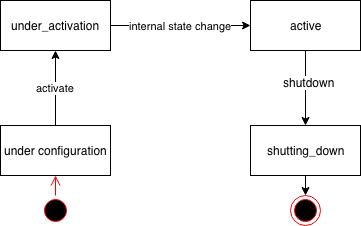
\includegraphics{images/ravnica}
	\caption{Simple State machine diagramm}
\end{figure}

\subsection{Data Structure}
The Data structure I used to implement Ravnica consists of a map with following entries:
\begin{itemize}
	\item \textbf{description} Saves the description which gets saved when starting a server
	\item \textbf{connections} Map for Handling the connections from one District to an other
	\item \textbf{creatures} Map for handling all the entered/active creatures on a Server
	\item \textbf{trigger} Set a trigger for a district
\end{itemize}

\subsection{All states}
Messages which get accepted in all states.
\subsubsection{get\_description}
Gets the description \texttt{Desc} which gets set on create of a District.

\subsection{Under configuration}
As soon as a Server started it is in the under\_configuration state.
\subsubsection{connect}
Connects 2 District with a Action, by saving it in the \texttt{connections} map, 
connects can only be made while district is under configuration in other states an error gets returned.

\subsubsection{trigger}
Under configuration also a trigger can be added to the server, here always the last one gets taken (overwritting whit the newest one).
Trigger gets rung whenever a creature enters or leaves a district.

\subsection{Under activation}
When \texttt{activate} gets called the district and it's neighbors need to get activated, under\_activation is a intermediate state until all neighbors and the district itself are activated.
In case the neighbors can't be activated (for example when a neighbor got shutdown), then the server goes back to the state of under\_configuration.

\subsubsection{activate}
Activate tries to activate all it's neighbors and changes the state of the server to \texttt{active} or back to \texttt{under\_configuration}.

\subsection{Active}
In the active state, no more new connections can be added, also no triggers.
So as soon as a district and it's neighbors is activated, it should only be possible to either run \texttt{get\_description}, \texttt{enter} or \texttt{take\_action} and of course shutting down.

\subsection{Shutting down}
When shutting down is called all neighbors of a district will be shut down as well and this can be propagated until all districts and it's nieghbors are shutdown.

\subsubsection{shutdown}

\subsection{Territories with cycle}

%\section{Solution}
%\subsection{Files}
%\subsection{Running the programm}
%\subsection{Running the tests}
%\section{Implementation}
%\subsection{Gen-Statem}

%\subsection{Data Structure}
%\subsection{All states}

%\section{Assessment}

%\subsection{Scope of Test Cases}

%\subsection{Correctness}

%\subsection{Code Quality}

\appendix
\section{Code Listing}
\subsection{Question 1.1: handin/appm/src/Utils.hs}
\label{appendix:question1-1}
\inputminted{haskell}{handin/appm/src/Utils.hs}
\subsection{Question 2.1: handin/ravnica/district.erl}
\inputminted{erlang}{handin/ravnica/district.erl}
%\inputminted{erlang}{handin/src/quizmaster_helpers.erl}

\end{document}